\documentclass[titlepage]{article}
\usepackage[margin=3cm]{geometry}
\usepackage{datetime}
\usepackage{fontspec}
\usepackage{graphicx}
\usepackage{hyperref}
\usepackage{kotex}
\usepackage[lighttt]{lmodern}
\usepackage{listings}
\usepackage{tikz}
\usepackage{sectsty}
\usepackage[edges]{forest}
\usepackage{float}
\usepackage{flowchart}

\usepackage[headsepline]{scrlayer-scrpage}
\newcommand{\doctitle}{CSED101: Assignment 1}
\clearpairofpagestyles
\ohead{\thepage}
\ihead{\doctitle}

\usetikzlibrary{arrows}
\usetikzlibrary{fit}

\setmainhangulfont{Noto Serif CJK KR}[
  UprightFont=* Light, BoldFont=* Bold,
  Script=Hangul, Language=Korean, AutoFakeSlant,
]
\setsanshangulfont{Noto Sans CJK KR}[
  UprightFont=* DemiLight, BoldFont=* Medium,
  Script=Hangul, Language=Korean
]
\setmathhangulfont{Noto Sans CJK KR}[
  SizeFeatures={
    {Size=-6,  Font=* Medium},
    {Size=6-9, Font=*},
    {Size=9-,  Font=* DemiLight},
  },
  Script=Hangul, Language=Korean
]
\lstset{
  numbers=none, frame=single, showspaces=false,
  showstringspaces=false, showtabs=false, breaklines=true, showlines=true,
  breakatwhitespace=true, basicstyle=\ttfamily, keywordstyle=\bfseries, basewidth=0.5em
}
\allsectionsfont{\sffamily}

\title{\doctitle}
\author{무은재학부 손량 (20220323)}
\date{Last compiled on: \today, \currenttime}

\begin{document}

\makeatletter
\begin{titlepage}
  \begin{center}
    \vspace*{3cm}
    \Huge
    \textsf{\@title}

    \vspace{1.5cm}
    \LARGE
    \@author

    POVIS ID: \texttt{ryangsohn}

    \vspace{0.5cm}
    담당 교수: 윤은영 교수님

    \vfill
    \large
    \textit{``나는 이 프로그래밍 과제를 다른 사람의 부적절한 도움 없이 완수하였습니다.''}
  \end{center}
\end{titlepage}

\section{문제의 개요}

본 프로그램은 `더 지니어스: 룰 브레이커'에서 플레이된 게임인 `인디언 홀덤' 게임을 C언어로 구현한 것이다. 사용자는 간단한 알고리즘을 기반으로 게임을 수행하는 컴퓨터와 대결할 수 있다. 이 프로그램에서 사용하는 structure chart는 다음과 같다.

\begin{figure}[H]
  \centering
  \begin{forest}
    for tree={
      draw,
      align=center
    },
    forked edges,
    [ASSN1: 인디언 홀덤
      [\texttt{card\_shuffle}
        [\texttt{rand\_range}
        ]
      ]
      [\texttt{user\_turn}
        [\texttt{is\_valid\_num}
        ]
      ]
      [\texttt{computer\_turn}
        [\texttt{min}
        ]
      ]
      [\texttt{calc\_winner}
        [\texttt{calc\_hand}
        ]
      ]
      [\texttt{print\_card\_info}
      ]
    ]
  \end{forest}
\end{figure}

\section{프로그램 구조 및 설명}

본 프로그램에서 사용한 알고리즘을 pseoudocode로 나타내면 다음과 같다.

\begin{lstlisting}
set random seed to current time
create variables round = 1, user_chips = 50, computer_chips = 50, past_winner = 1
infinite loop:
  if round > 10 or user_chips * computer_chips == 0:
    break
  if round != 1:
    clear the screen
  shuffle cards and print game status
  print game status and card info
  calculate winner according to current cards
  if user_chips > 1 and computer_chips > 1:
    create variable turn_count = 0
    infinite loop:
      print currently betted chip counts
      create variable turn = 1 - (past_winner + turn_count) % 2
      if turn == 0:
        do user betting turn
      else:
        do computer betting turn
      if current player folded:
        set winner to opponent
        break
      if current player called:
        break
  reveal user card
  print winner
  set past_winner = winner
  print chips left
  increment round by 1
decrement round by 1
print number of games played, which is round
print remaining chips
print winner
\end{lstlisting}

Flowchart로 나타내면 다음과 같다.

\begin{figure}[H]
  \centering
  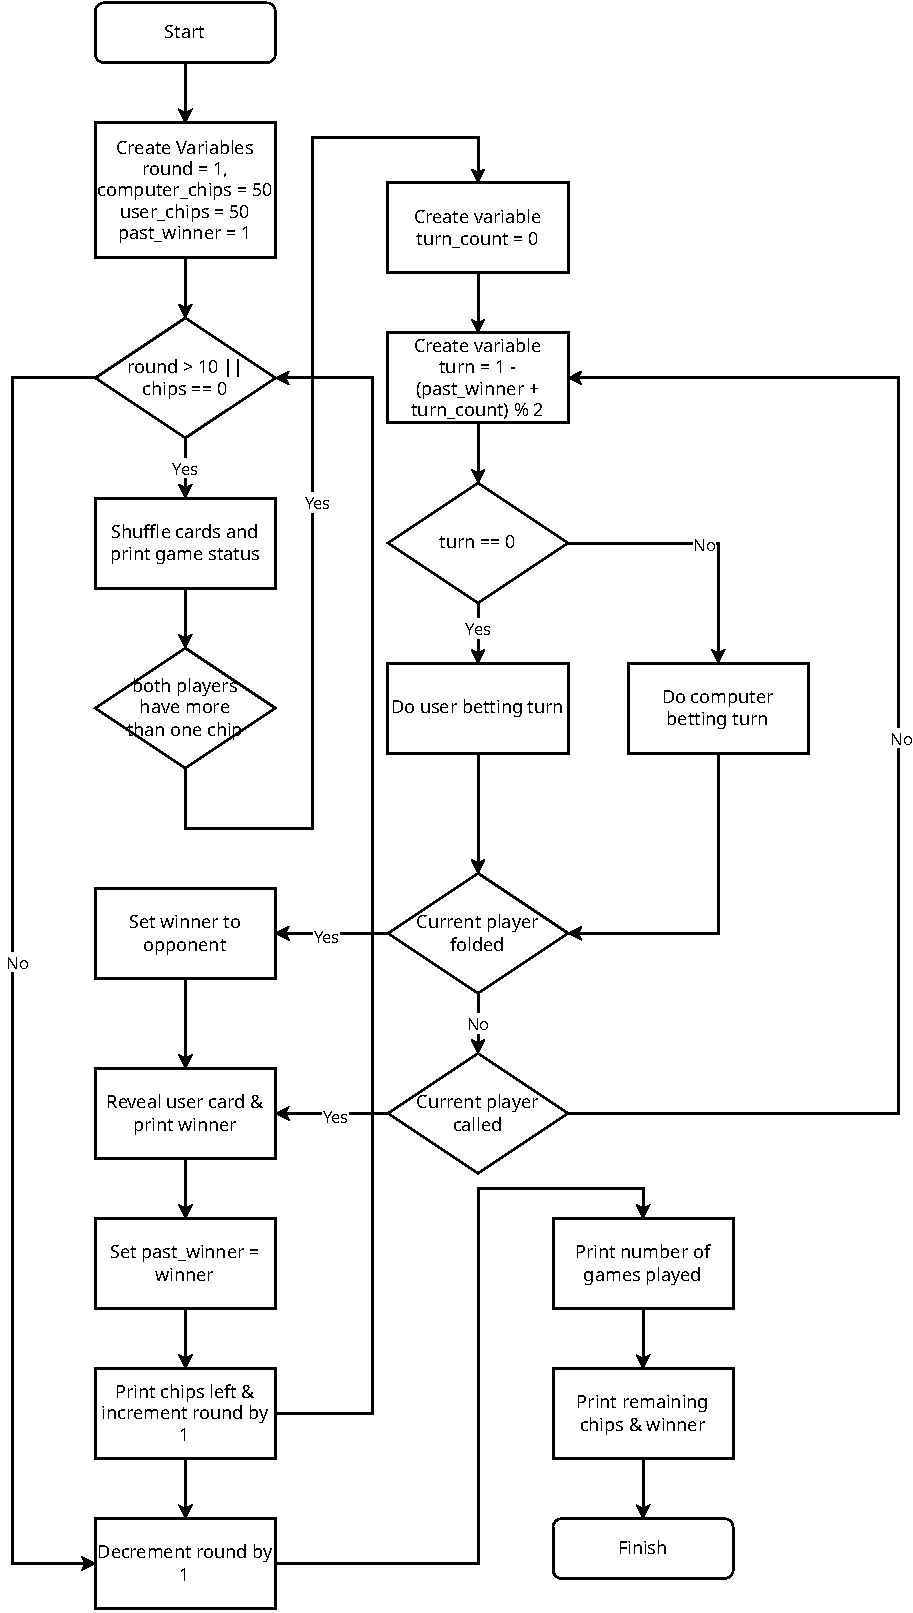
\includegraphics[width=0.7\linewidth]{flowchart.drawio.pdf}
\end{figure}

\section{프로그램 실행 방법과 예제}

첨부한 \texttt{assn1.c} 파일은 Linux, macOS 등의 UNIX 계열 OS에서 실행하는 것을 전제로 작성되었다.\footnote{Windows의 경우 WSL이나 Cygwin 등의 환경에서 실행할 수 있을 것이다.} \texttt{gcc} 컴파일러가 설치된 환경에서는 다음 명령어를 통해 코드를 컴파일할 수 있다.

\begin{lstlisting}
$ gcc -o assn1 assn1.c
\end{lstlisting}

이때 프로그램을 실행한 모습은 다음과 같다.

\begin{figure}[H]
  \centering
  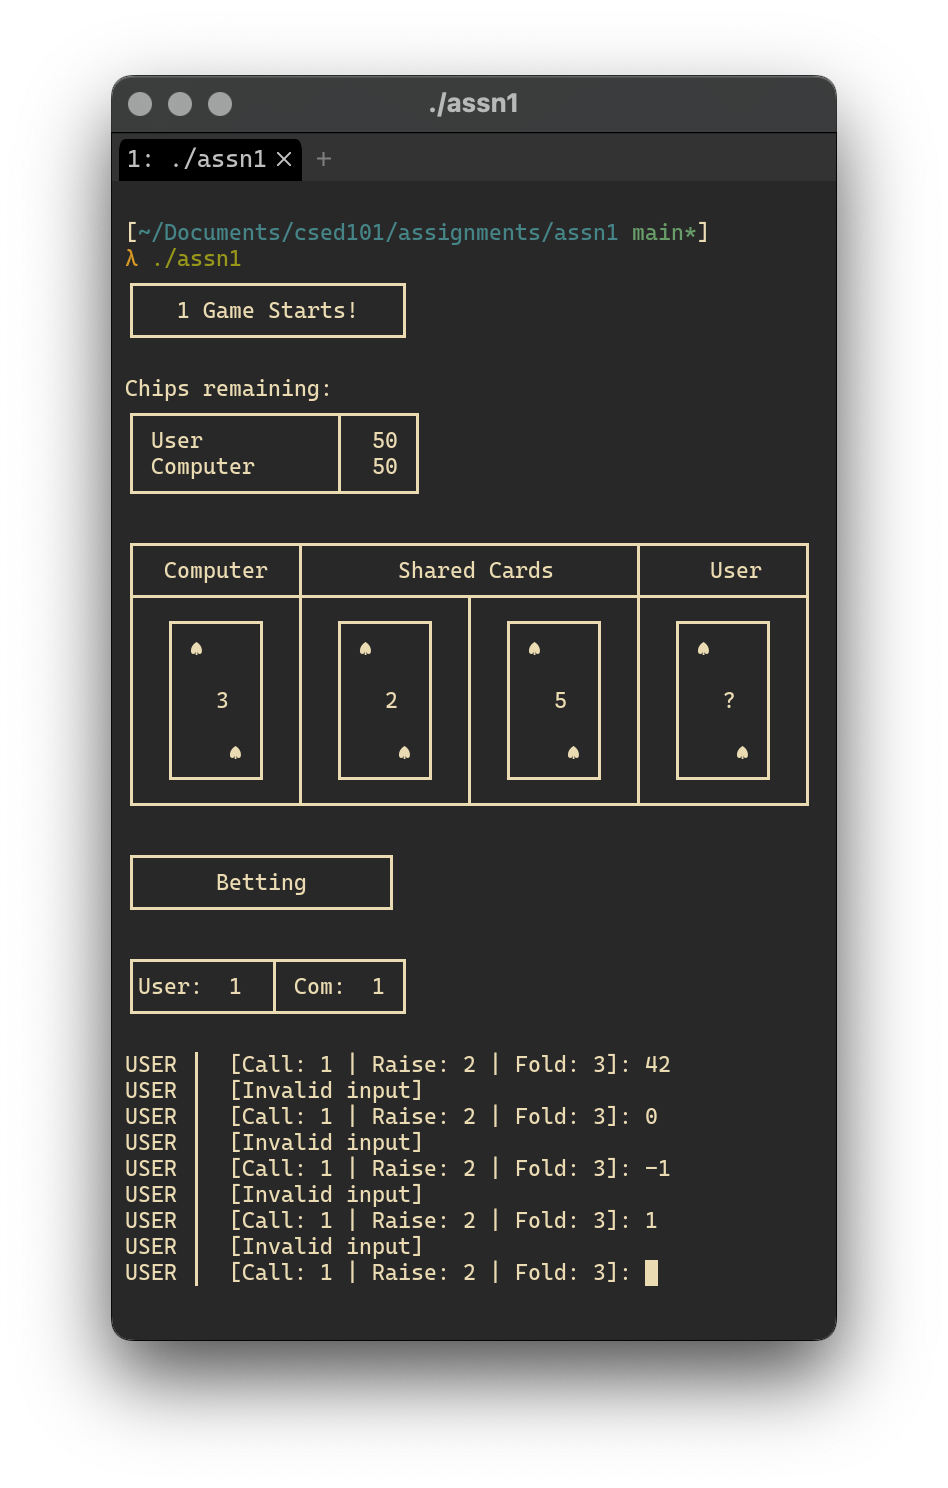
\includegraphics[width=0.6\linewidth]{invalid-input.png}
  \caption{사용자의 잘못된 입력에 대해 메시지를 출력하는 모습}
\end{figure}

\begin{figure}[H]
  \centering
  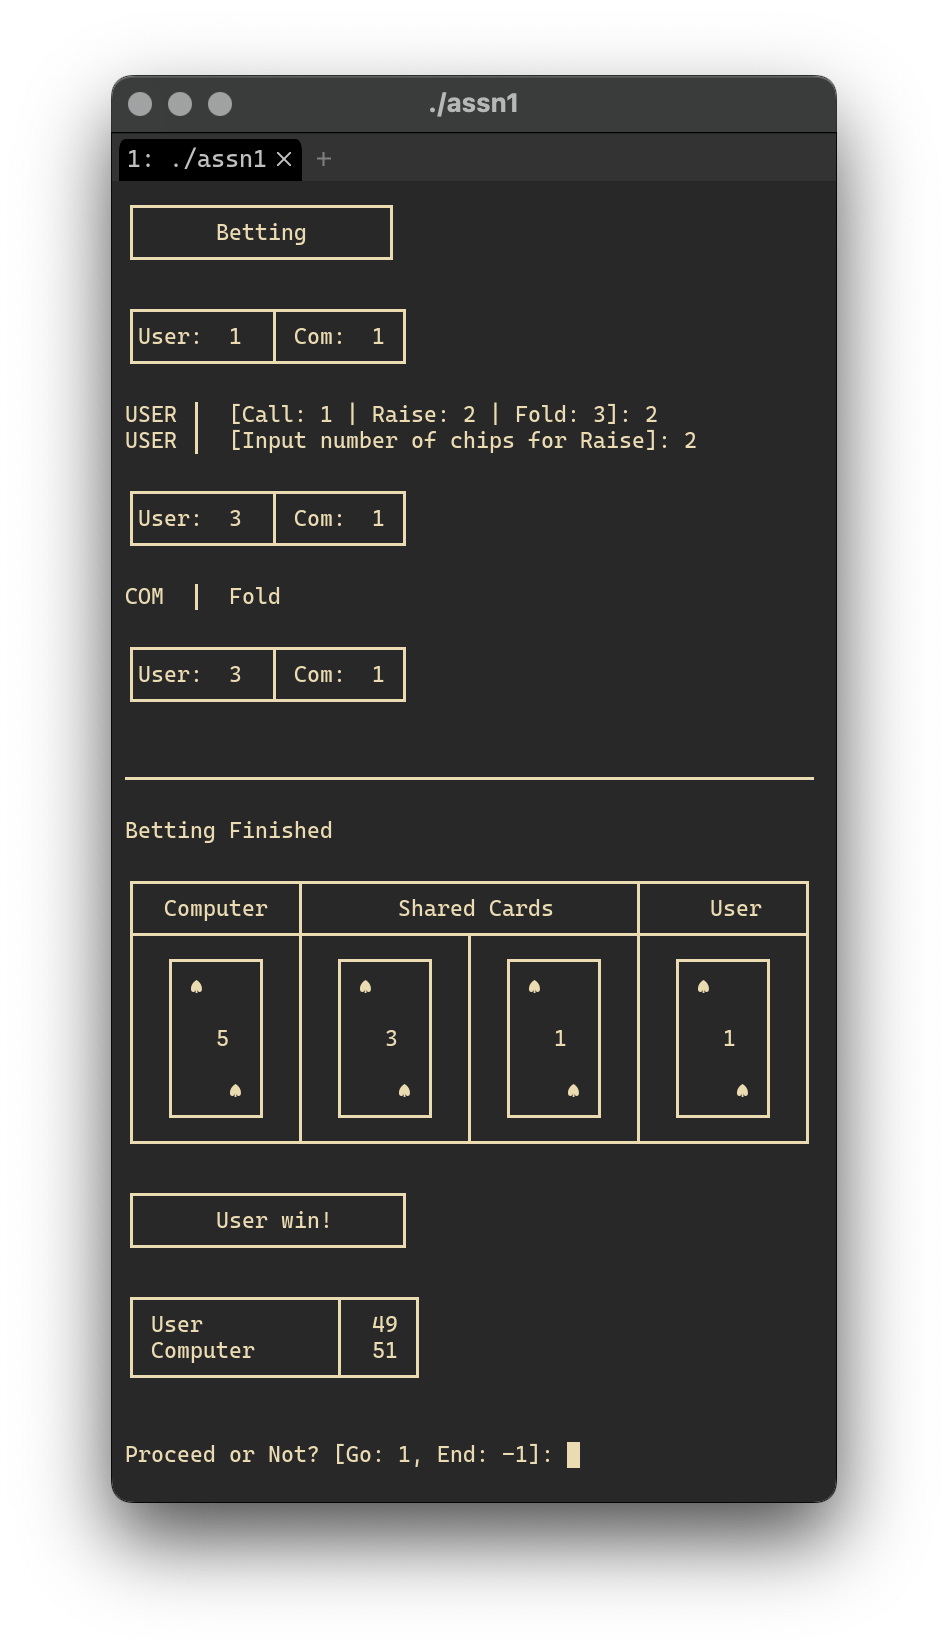
\includegraphics[width=0.6\linewidth]{betting.png}
  \caption{베팅이 진행되는 모습. 컴퓨터가 fold를 선택하여 사용자가 승리하였다.}
\end{figure}

\begin{figure}[H]
  \centering
  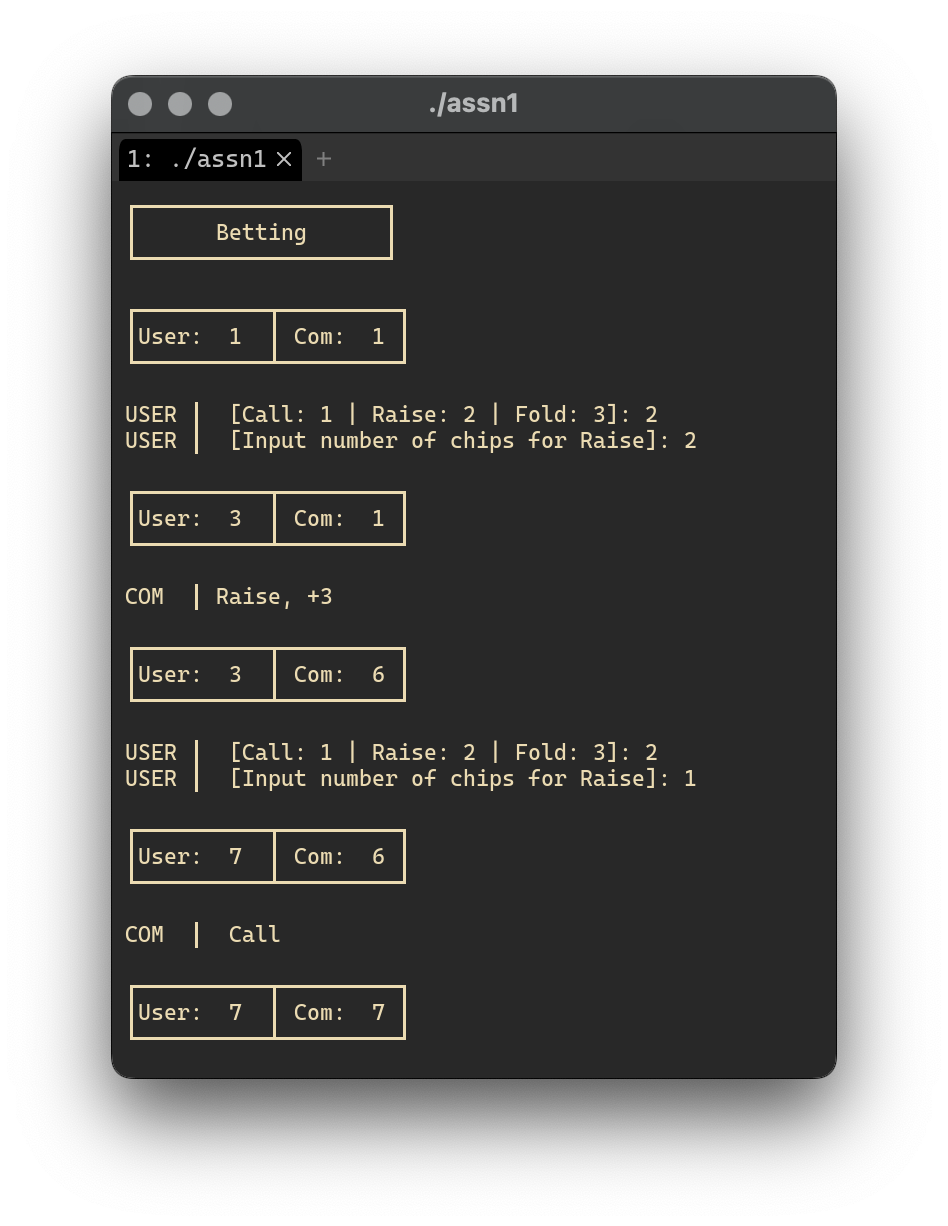
\includegraphics[width=0.6\linewidth]{betting-long.png}
  \caption{베팅이 길게 진행되는 예시.}
\end{figure}

\begin{figure}[H]
  \centering
  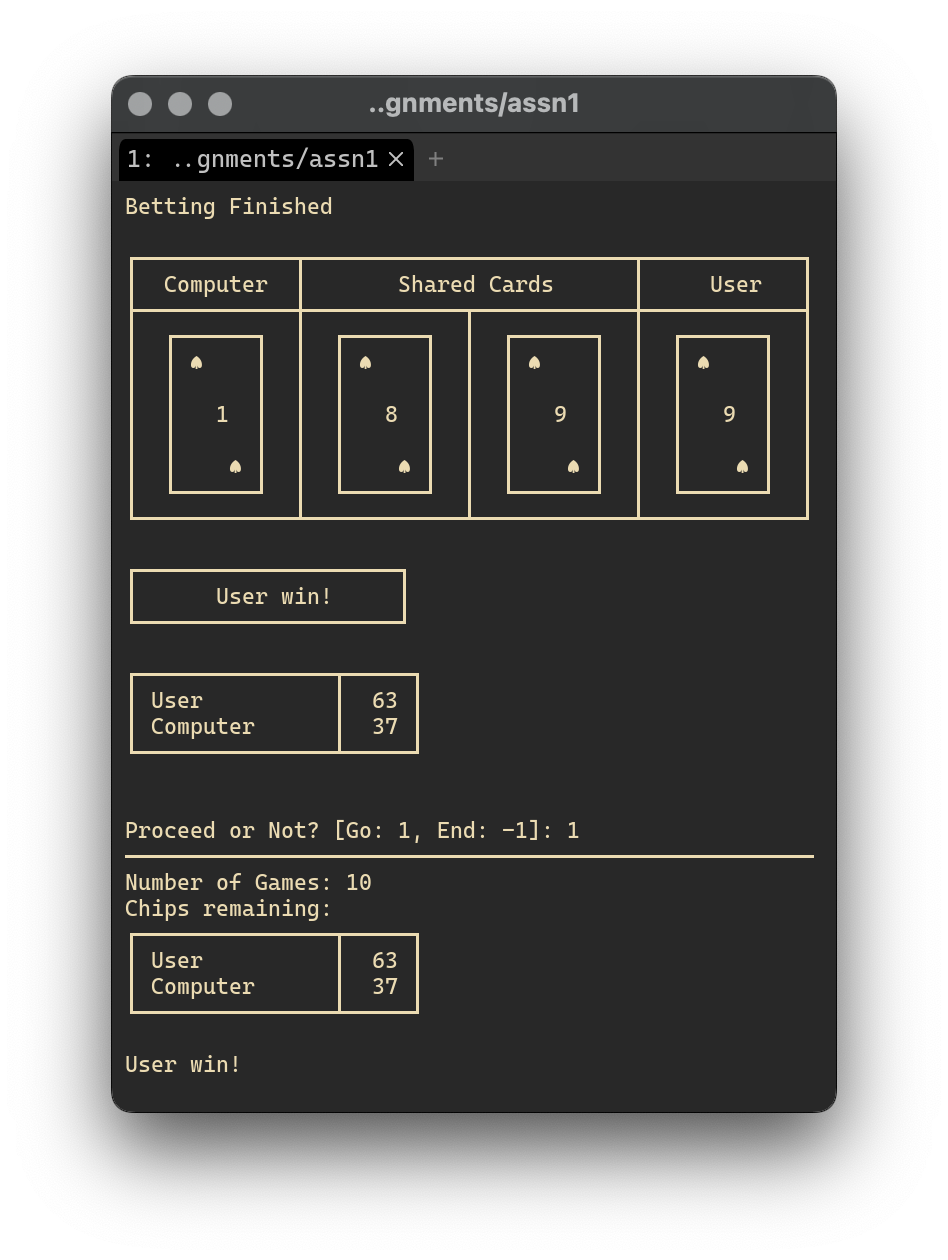
\includegraphics[width=0.6\linewidth]{gameover.png}
  \caption{게임 종료 시의 메시지.}
\end{figure}

\section{토론}

\subsection{각 턴에서의 선공, 후공 결정}

유저가 무조건 선공인 첫 게임을 제외하고, 이전 게임에서 진 사람이 선공을 가져간다는 룰을 구현하기 위해서 나머지 연산을 사용하였다. 적절히 상수를 선언하여 유저에 해당하는 값을 0, 컴퓨터에 해당하는 값을 1로 정하였다. 이전 게임의 승자를 저장하는 변수와 현재 게임의 턴 수를 더하고 2로 나누면, 턴 수 또는 이전 게임의 승자가 바뀔 때마다 0, 1이 번갈아 바뀜을 이용하여 각 턴에서 어떤 플레이어가 베팅할지를 정할 수 있었다.

\subsection{랜덤 함수의 직관적인 사용}

프로그래밍 시간에 배웠듯 반열린 구간 \([a, b)\)의 랜덤한 숫자는 \texttt{rand() \% (b - a) + a}의 코드로 생성할 수 있다. 하지만 이러한 코드가 프로그램 곳곳에 있으면 가독성이 떨어질 수도 있기 때문에, 랜덤한 숫자를 생성하는 함수인 \texttt{rand\_range(a, b)} 함수를 정의하여 코드 곳곳에서 사용하였다.

\section{결론과 개선 방향}

변수 선언, 함수 실행, 포인터 등 C언어의 기본적인 문법과 \texttt{scanf}, \texttt{printf}, \texttt{rand} 등의 표준 라이브러리 함수들을 사용하여 인디언 홀덤 게임을 구현하였다. 구현된 프로그램은 잘 작동하지만, 몇 가지 부족한 점을 여기서 살펴볼 것이다.

\subsection{컴퓨터의 전략}

컴퓨터의 전략은 게임으로서 이 프로그램의 성공을 좌지우지할 수 있는 중요한 요소이다. 현재 컴퓨터의 전략은 단순히 상대의 패를 보고, no pair 상태인지만 확인한 다음 미리 정해진 확률에 따라 베팅한다. 하지만 이 경우 사용자 입장에서는 매우 `재미 없게' 이길 확률이 상당히 높다. 나온 카드를 기반으로 승률을 계산하여 그에 따라 베팅하는 전략을 코딩한다면, 좀 더 재미있는 게임이 나올 것으로 보인다. 나아가, 네트워크를 통해 다른 컴퓨터와 연결하여 멀티플레이를 하는 기능도 있으면 좋을 것이다.

\subsection{유저 인터페이스 관련 코드}

현재 코드에서 화면에 출력하는 함수에는 출력 상황(칩 수 출력, 카드 출력 등) box drawing character로 그린 그래픽이 하드코딩되어 있다. 이러한 방식으로 구현되어 있으면 프로그램의 유지 보수가 어려워지기 때문에, 출력될 그래픽의 구조를 함수에 적당한 자료구조를 통해 입력하면 화면에 렌더링하는 알고리즘이 필요할 것으로 보인다.

\end{document}
